\subsection{Unsupervised Learning}

\indent 

\noindent \textbf{Supervised Learning}:

Given a dataset with features/predictors $(X_{i1},X_{i2},...,X_{ip})$ and a target outcome variable $(Y_i)$, the goal is to learn a model $f(X_{i1},...,X_{ip})$ to explain/predict the target.

\noindent \textbf{Unsupervised learning}:

Given a dataset with features $(X_{i1},X_{i2},...,X_{ip})$, the goal is to visualise, find patterns, subgroups/clusters within the data.

\subsection{Clustering}

\subsubsection{Overview}

\indent 

\noindent\textbf{Clustering}:

Groups similar observations based on a \textbf{similarity measure}.

\noindent\textbf{Clustering Goals}:

\begin{itemize}
    \item \textbf{Compact Clusters}: Observations within a cluster should be close together.
    \item \textbf{Well-Separated Clusters}: Observations from different clusters should be far apart.
\end{itemize}

\subsubsection{Typical methods}

\noindent\textbf{Partitioning}:

\begin{itemize}
    \item Pre-specified number $K$ of mutually exclusive and exhaustive groups.
    \item Iterate until criteria is met
\end{itemize}

\noindent\textbf{Hierarchical methods}:

\begin{itemize}
    \item Agglomerative: Bottom up, more popular
    \item Divisive: Top down, less popular
    \item Display results with dendrogram
\end{itemize}

\subsubsection{$K$-Means Clustering}

\noindent\textbf{Measuring Cluster Compactness}:

For cluster $C_k$, we can define within-group sum of squares as:

\begin{align*}
    \text{WSS}_k = \frac{1}{|C_k|}\sum_{i,j\in C_k}||x_i - x_j||^2, k = 1,...,K
\end{align*}

This is the sum of all the pairwise squared Euclidean distances between observations in the $k^{th}$ cluster, divided by total number of observations in the $k^{th}$ cluster.

$\sum_{i,j \in C_k}||x_i - x_j||^2$ is the sum of all the pairwise squared Euclidean distances between observations in the $k^{th}$ cluster.

$|C_k|$ is the total number of observations in the $k^{th}$ cluster.

\bigskip

\noindent\textbf{Clustering Objective}:

To minimize the total within-group sum of squares criterion.

\begin{align*}
    \text{WSS}_{\text{Total}} = \sum_{k=1}^{K}\text{WSS}_k
\end{align*}

The total within sum of square criterion will \textbf{decrease} as $K$ increases.

Rule of thumb: Look for the elbow.

\begin{figure}[h]
    \centering
    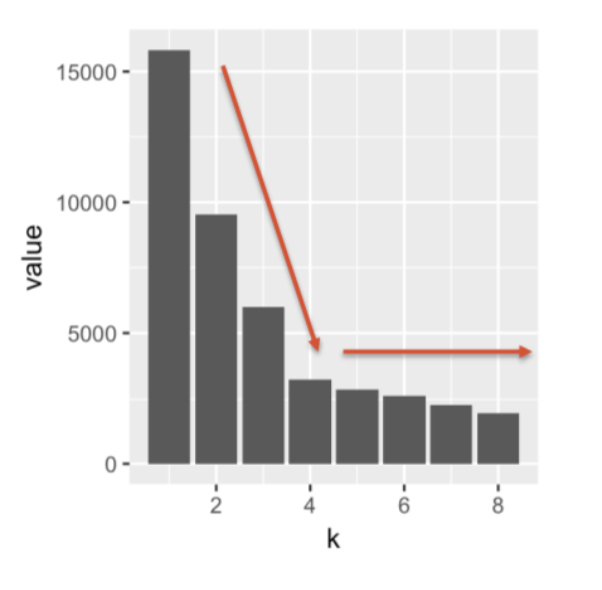
\includegraphics[width=0.5\linewidth]{Figure/Week 4/Elbow.png}
    \caption{Elbow Plot}
\end{figure}

\bigskip

\noindent\textbf{Process}:

Initialise each observation at random to a cluster.

Iterate the following until the assignments stop changing:

\begin{itemize}
    \item For each of the $K$ clusters, compute the cluster centroid.
    \item Assign each observation to the cluster whose centroid is closest (where the closest is defined using the Euclidean distance).
\end{itemize}

\bigskip 

\noindent\textbf{Properties}:

\begin{itemize}
    \item The number of clusters $K$ needs to be specified.
    \item Local solution and not necessarily global solution.
    \item Depends on starting values (the random starting values)-run the algorithms multiple times.
    \item Best for compact, spherical clusters.
    \item Does not work well when cluster sizes are different.
\end{itemize}

\subsubsection{Hierarchical clustering}

\indent 

Begin with every observation representing a single cluster.

At each iteration, merge the two closest clusters into one cluster:

\begin{itemize}
    \item Needs \textbf{a measure of similarity/dissimilarity} between two clusters
    \item These measures are called \textbf{linkages}.
\end{itemize}

\noindent\textbf{Linkages}: 

Measure of dissimilarity between two sets of objects that determine how two set of objects are merged.

\begin{itemize}
    \item Single linkage
    \item Complete linkage
    \item Average Linkage
\end{itemize}

\begin{figure}[h]
    \centering
    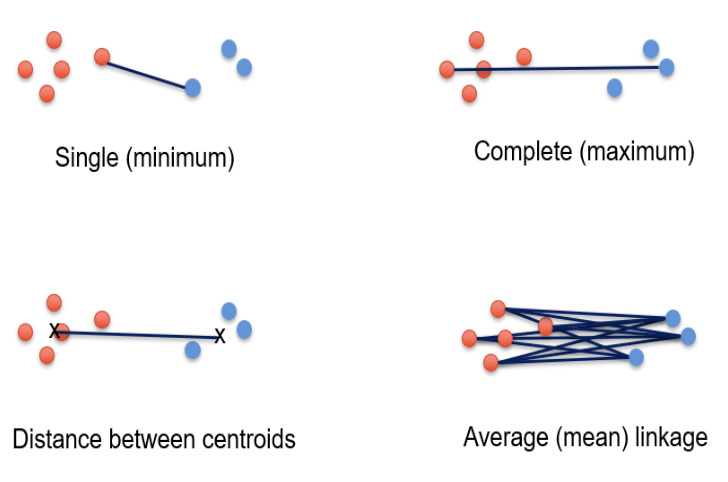
\includegraphics[width=0.8\linewidth]{Figure/Week 4/Linkages.png}
\end{figure}

\subsection{Principal Components Analysis (PCA)}

\indent 

Suppose we have a data matrix $X$ with $n$ observations and $p$ features. Principal Component Analysis (PCA) helps us reorganise/transform the data into a new coordinate system. The data still has $p$ dimensions, but in a new set of axes. The goal is to capture most of the variation using just the first few dimensions, making the data easier to analyse.

\subsubsection{High-dimensional data}

High-dimensional data refers to data set with more features $p$ than observations $n$.

It is very hard to visualize high-dimensional data. Only have 2 (sometimes 3 or 4) dimensional canvas to create plots. Many algorithms and methods have been designed for low dimensional data and would not work well for high-dimensional data.

\subsubsection{Dimension reduction strategies}

\indent 

\noindent\textbf{Eliminate or remove features}

\noindent\textbf{Select features} (Example: Lasso and ridge regression)

\noindent\textbf{Build or construct new features from existing ones}

\begin{itemize}
    \item Replace many existing features with a single one.
    \item PCA and $t$-SNE
\end{itemize}

\subsubsection{Principal components}

\indent 

\begin{figure}[h]
    \centering
    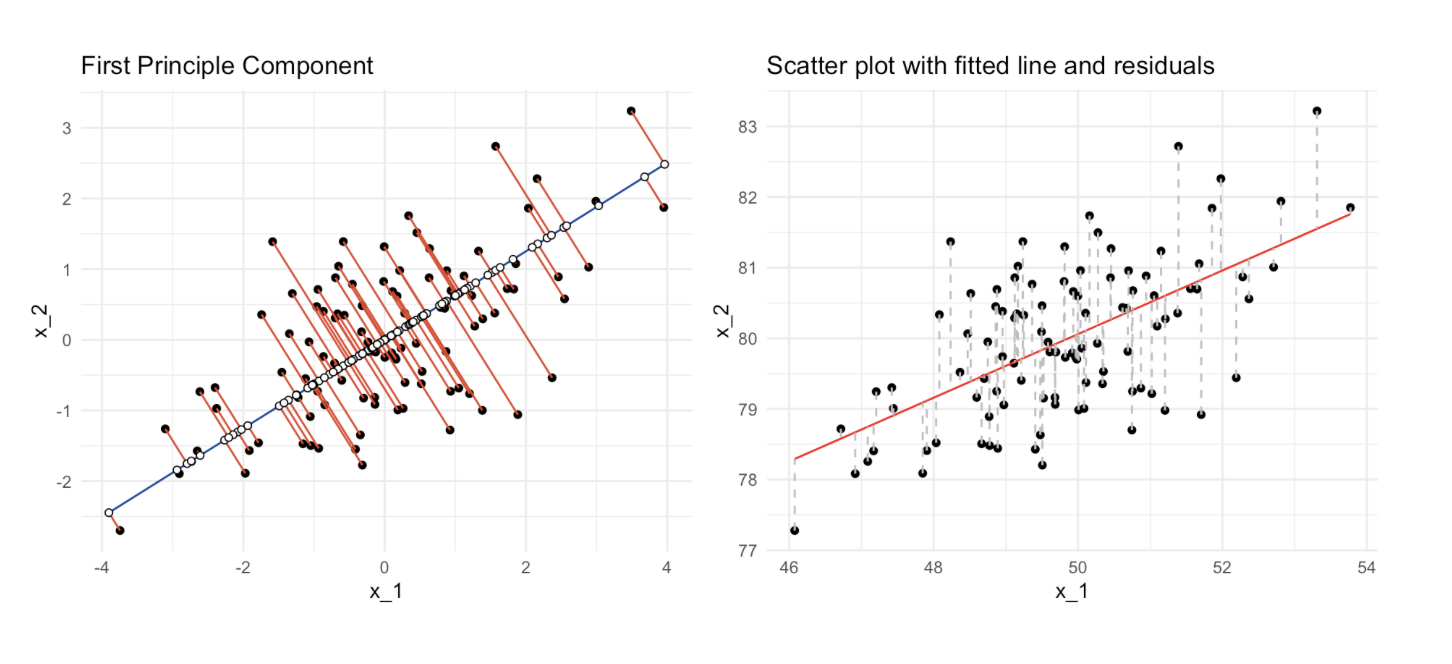
\includegraphics[width=0.8\linewidth]{Figure/Week 4/Geometric.png}
    \caption{Geometric interpretation}
\end{figure}

Start with a data matrix $\boldsymbol{X}$, and assume it has \textbf{mean zero}.

\begin{align*}
    \boldsymbol{X} = (X_1,X_2,...,X_n)
\end{align*}

The first principal component is the \textbf{normalised linear combination of the features} that \textbf{maximises the variance} in the new component.

\begin{align*}
    & Z_1 = \phi_{11}X_1+\phi_{21}X_2+...+\phi_{p1}X_p = \sum_{j=1}^{p}\phi_{j1}X_j = \boldsymbol{X}\boldsymbol{\phi}_{1}\\
    & \boldsymbol{\phi}_1 = (\phi_{11},...,\phi_{p1})^T
\end{align*}

The elements $\phi_{j1}$ are known as the loadings of the first principal component.

By normalised, we mean the squared loadings have to sum to 1:

\begin{align*}
    \sum_{j=1}^p\phi_{j1}^2 = 1 \iff \boldsymbol{\phi}_1^T\boldsymbol{\phi}_1 = 1
\end{align*}

It is desired to maximise the sample variance of $Z_{i1},...,Z_{n1}$, where $Z_{i1}$is the $i-th$ componenet of $Z_1$:

\begin{align*}
    \frac{1}{n-1}\sum_{i=1}^n(\sum_{j=1}^p\phi_{j1}x_{ij})^2
\end{align*}

Given the principal component loadings, we can project our data matrix $\boldsymbol{X}$ onto the principal component space.

\noindent\textbf{Principal component score}: The projection is a linear combination of the sample feature values.

\begin{align*}
    z_{i1} = \phi_{11}x_{i1}+\phi_{21}x_{i2}+...+\phi_{p1}x_{ip}
\end{align*}

The first principal component score vector is:

\begin{align*}
    \boldsymbol{Z}_1 = (z_{11},z_{21},...,z_{n1})
\end{align*}

The principal component score vectors are uncorrelated (orthogonal).

\subsubsection{Preprocessing for PCA}

\indent 

In PCA, it’s common to center variables by subtracting the mean. You can also standardise them so all variables have a standard deviation of 1. Standardising ensures all variables contribute equally. Improves interpretability and prevents one variable from dominating the analysis.

\noindent \textbf{Why Standardisation}: Variables may have different units. This leads to different variances, affecting PCA results.

\noindent \textbf{Impact on Loadings}: PCA loadings give more weight to variables with higher variance. This can bias the analysis if some variables dominate.

\subsubsection{PCA Properties}

\begin{itemize}
    \item Unique and Global solution!
    \item Ordered components
    \item Best linear dimension reduction possible
    \item Is not the best for non-linear relationships
\end{itemize}

\subsubsection{PCA with $K$-means}

\indent 

Very common approach to deal with high dimensional data.

Use the first $M$ principal component scores as inputs into the $K$-means algorithm, where $M\ll p$.

Can help improve the clustering model if the signal in the data can be captured in a few principal components.

\subsubsection{PCA with regression}

\indent 

Use the first $M$ principal component scores as the predictors in a linear regression model.

We are assuming that a small number of principal components can explain most of the variability in the data as well as the response.

PCA is useful when variables in the data are highly correlated (i.e., collinear).

\subsection{Dimension reduction $t$-SNE}

\indent 

Non-linear technique developed for visualizing high dimensional datasets.

Use local structure in the data to find a low dimensional representation.

\subsubsection{$t$-SNE vs PCA}

\indent 

\begin{figure}[h]
    \centering
    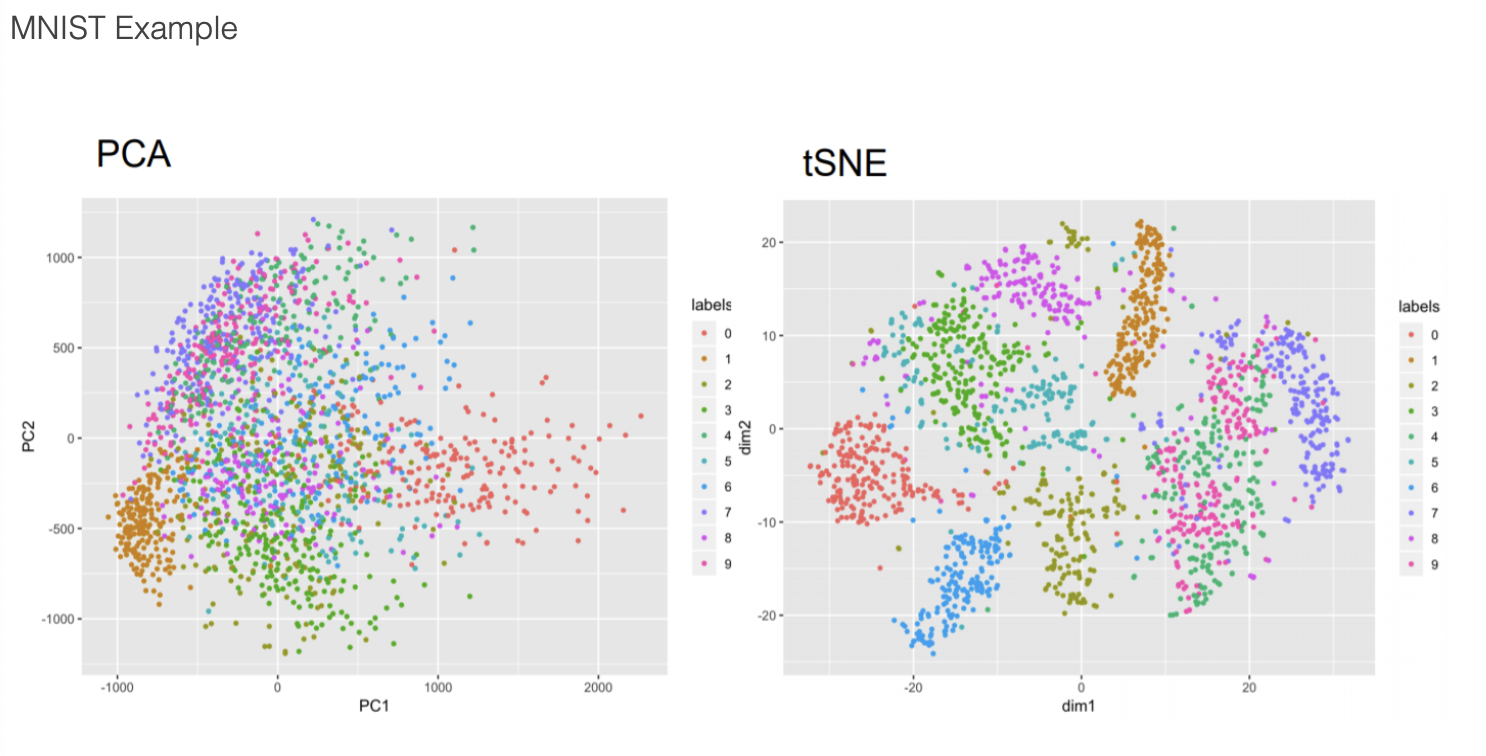
\includegraphics[width=0.8\linewidth]{Figure/Week 4/t-SNE VS PCA.png}
\end{figure}

\noindent\textbf{PCA}

\begin{itemize}
    \item PCA is a linear method and can only capture linear relationships.
    \item PCA is defined by a mathematical formula.
    \item The principal components (PCs) from PCA can be interpreted and used for inference.
    \item PCA is less computationally intensive
\end{itemize}

\noindent\textbf{$t$-SNE}

\begin{itemize}
    \item $t$-SNE is a non-linear technique and is able to find complicated non-linear relationships.
    \item $t$-SNE is a probabilistic method – it will give you a different representation every time you run it
    \item $t$-SNE is mostly a visualization method. The visualization from $t$-SNE cannot be used for inference.
    \item $t$-SNE is more computationally intensive
\end{itemize}

\subsection{Dimension reduction: Multidimensional Scaling (MDS)}

\indent 

Visually represent proximities (similarities or distances) between objects in a lower dimensional space (usually 2 or 3d space).

The objective of MDS is to take a Matrix of similarities or dissimilarities, $\boldsymbol{D}$, and find projections $z_1,...,z_k$ where $k$ is the desired lower dimension.

The distances are near preserved by optimizing a stress function.

Full data not required.

\subsubsection{MDS Stress functions}

\indent 

These functions attempt to force the lower dimensional projections to preserve the distances in the original data.

\noindent\textbf{Commoon stress functions}:

\begin{align*}
    \text{Least Squares:}S_{LS}(z_1,z_2) = \sqrt{\sum_{i\neq j}(d_{ij} - ||z_i-z_j||)^2}
\end{align*}

\subsubsection{Comments on MDS}

\indent 

\noindent\textbf{Pros \& Cons}:

\begin{itemize}
    \item Requires only a distance or dissimilarity matrix, not the full dataset.
    \item Must choose the number of dimensions KK (similar to the elbow method in a Scree plot).
    \item Useful for visualizing non-linear data in a lower-dimensional space.
\end{itemize}

\bigskip 

\noindent\textbf{How to Interpret MDS Maps}

\begin{itemize}
    \item Rotation does not matter – axes and orientation are arbitrary.
    \item Focus on relative positions – only distances between points are meaningful.
    \item Objects closer together on the MDS map are more similar based on the input distance matrix.
\end{itemize}